\documentclass[10pt]{beamer}

\usetheme{default} % theme général du diaporama

% paquets pour le français
\usepackage[T1]{fontenc}
\usepackage[utf8]{inputenc}
\usepackage{graphicx}
% Use quotes
\usepackage{csquotes}

% Set height of table rows relative to maximum
\renewcommand{\arraystretch}{1.25}

% Number figures
\setbeamertemplate{caption}[numbered]

% use serif font with rm
% \renewcommand{\familydefault}{\rmdefault}

\title{Spatially continuous identification of beta diversity hotspots using species distribution models}
\author{Gabriel Dansereau}

\begin{document}

\begin{frame}
  \titlepage
\end{frame}

\begin{frame}
  \frametitle{Objective}
  \begin{displayquote}
    "Spatially Continuous Identification of Beta Diversity Hotspots Using Species Distribution Models"
  \end{displayquote}
  \begin{figure}
    \centering
    \hspace*{0.0cm}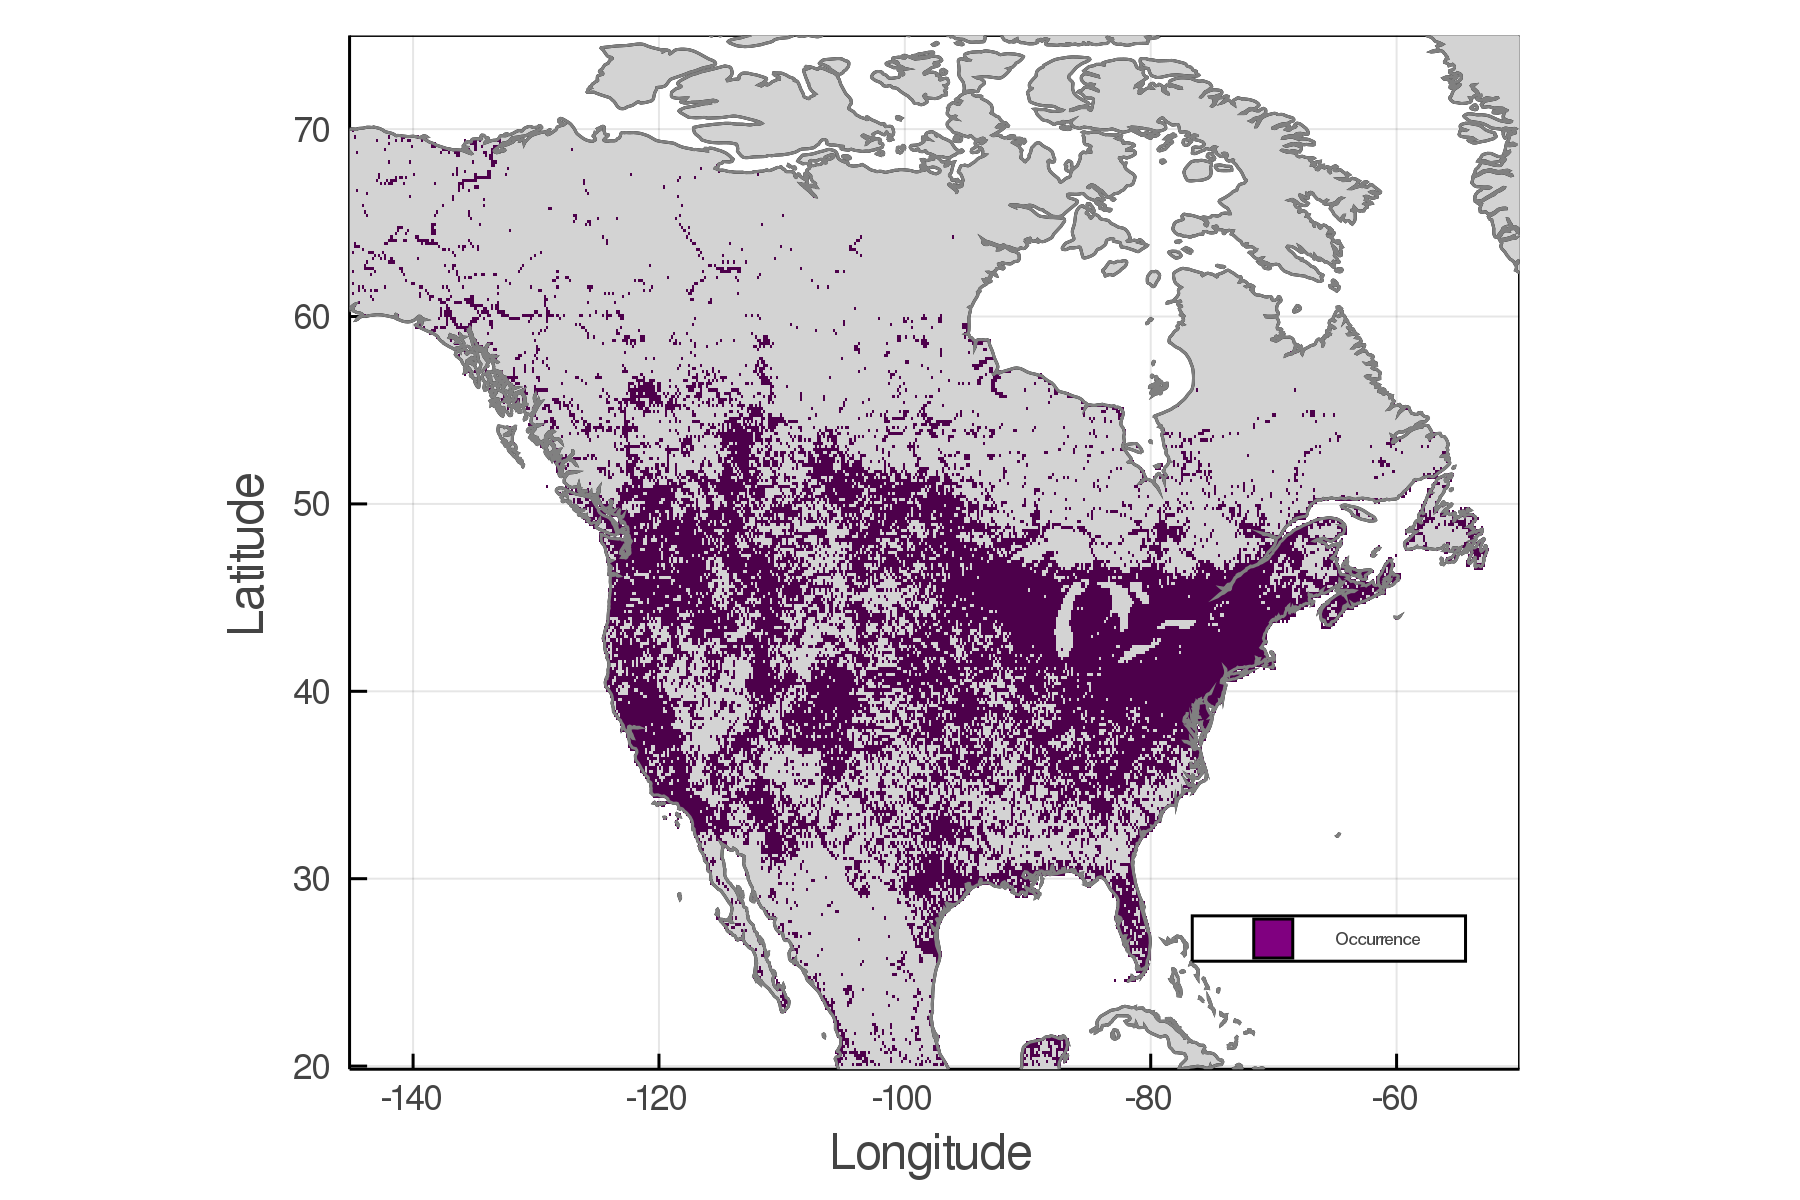
\includegraphics[scale=0.08]{fig/01_raw_singlesp.png}
    \hspace*{0.0cm}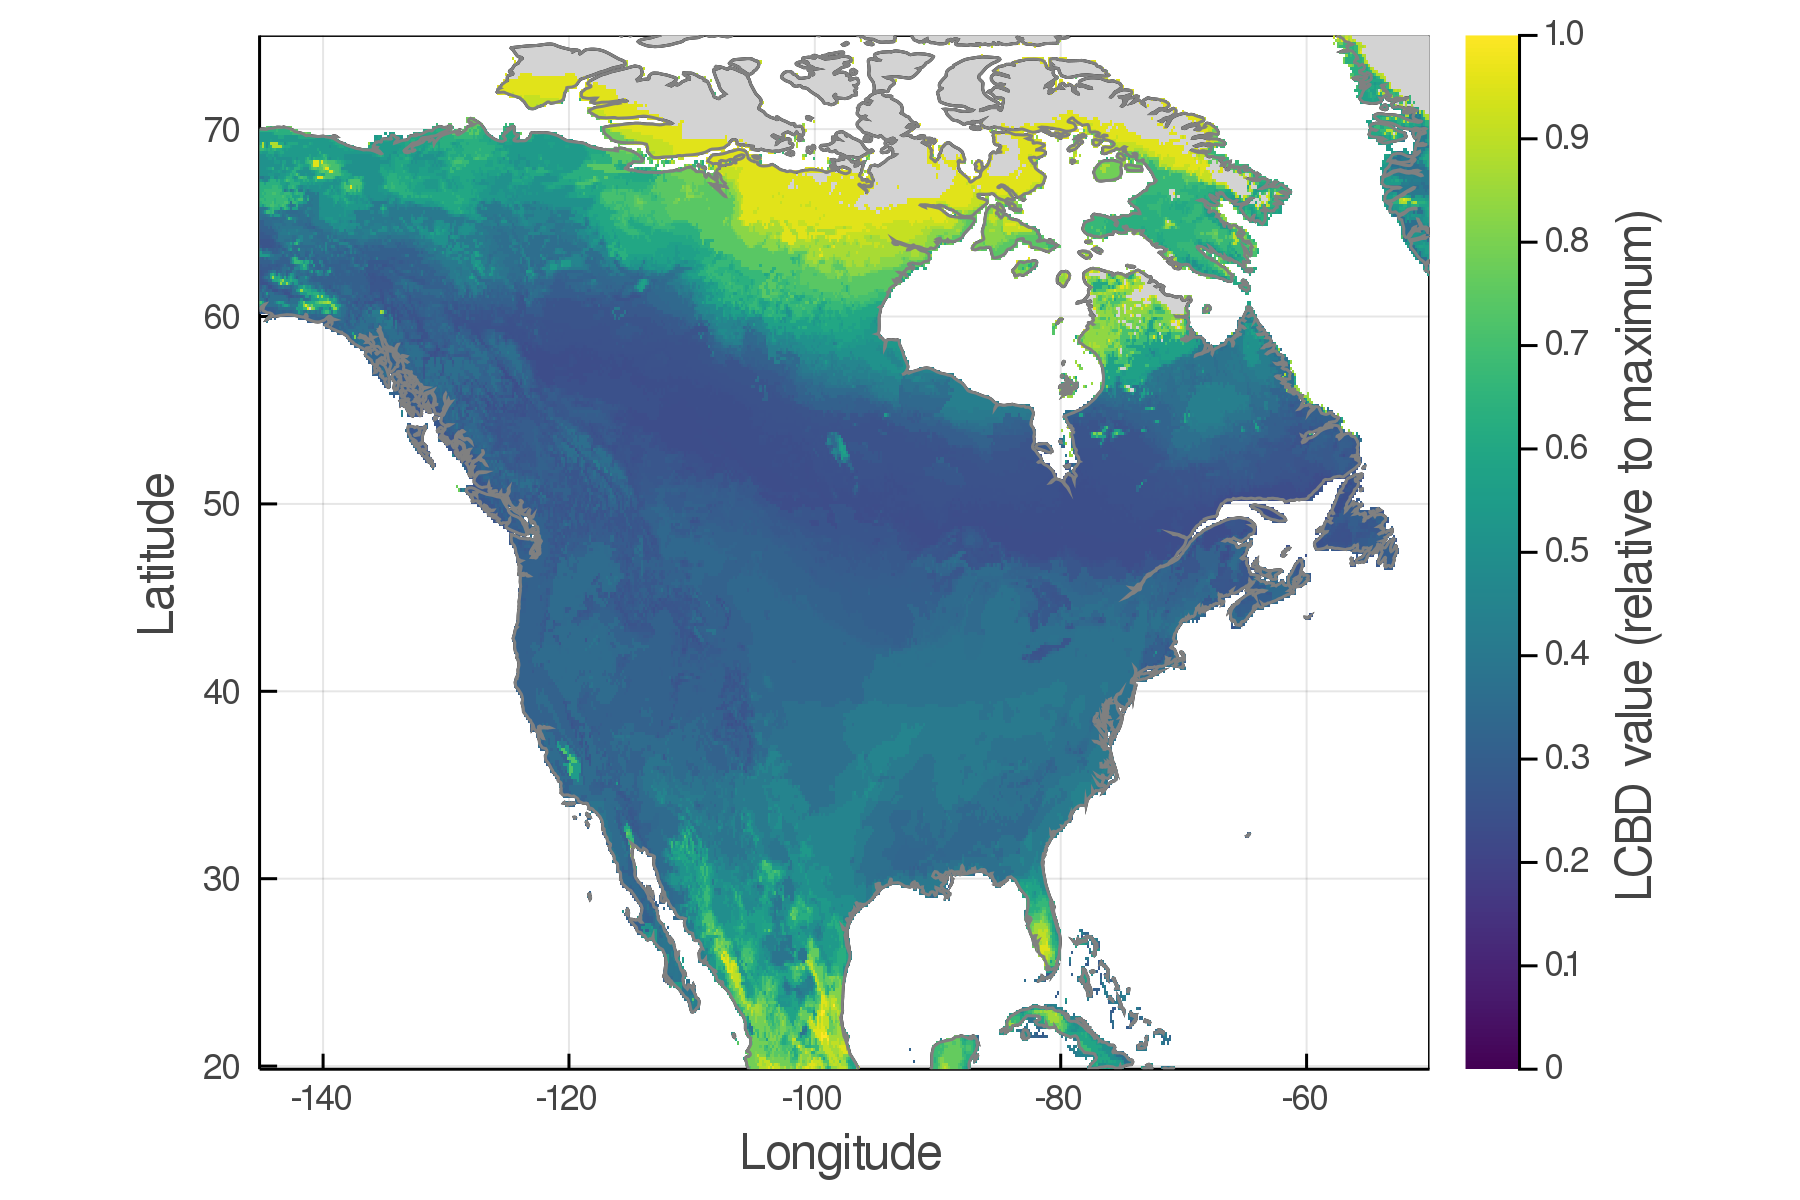
\includegraphics[scale=0.08]{fig/05_sdm_lcbd.png}
    \hspace{4.0cm}\begin{itemize}
      \item Beta diversity hotspots (LCBD)
      \item Species distribution models (SDM)
      \item Spatially continuous identification
    \end{itemize}
  \end{figure}
\end{frame}

\begin{frame}
  \frametitle{Ex 1. Discontinuous Identification of Beta Diversity Hotspots}
  \begin{figure}
    \centering
    \hspace*{-0cm}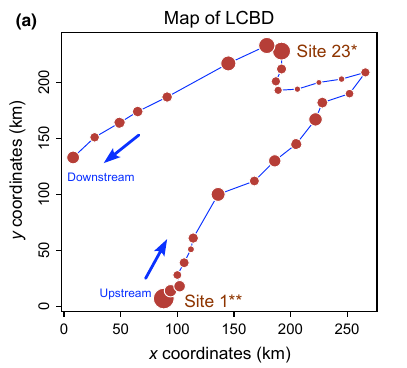
\includegraphics[scale=0.5]{fig/lcbd_LegeDeCa2013.png}
    \caption{Example of LCBD calculation on a river stream (Legendre \& De Caceres, 2013)}
  \end{figure}
\end{frame}

\begin{frame}
  \frametitle{Ex 2. Discontinuous Identification of Beta Diversity Hotspots}
  \begin{figure}
    \centering
    \hspace*{-0cm}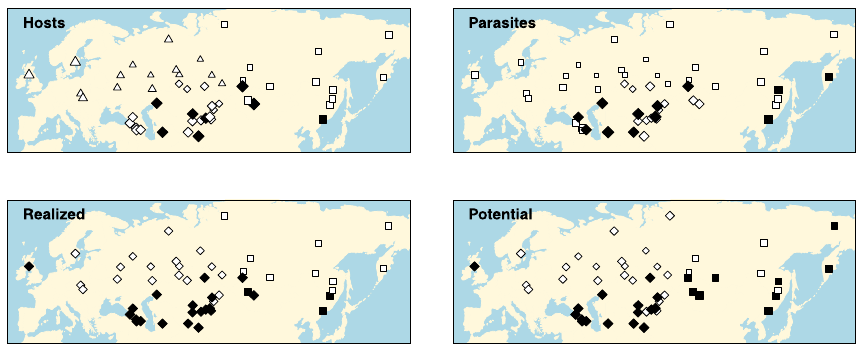
\includegraphics[scale=0.35]{fig/lcbd_Pois2017.png}
    \caption{Example of LCBD calculation on an extended scale (Poisot et al., 2017)}
  \end{figure}
\end{frame}

\begin{frame}
  \frametitle{Available Data}
  \begin{figure}
    \centering
    \hspace*{-0.5cm}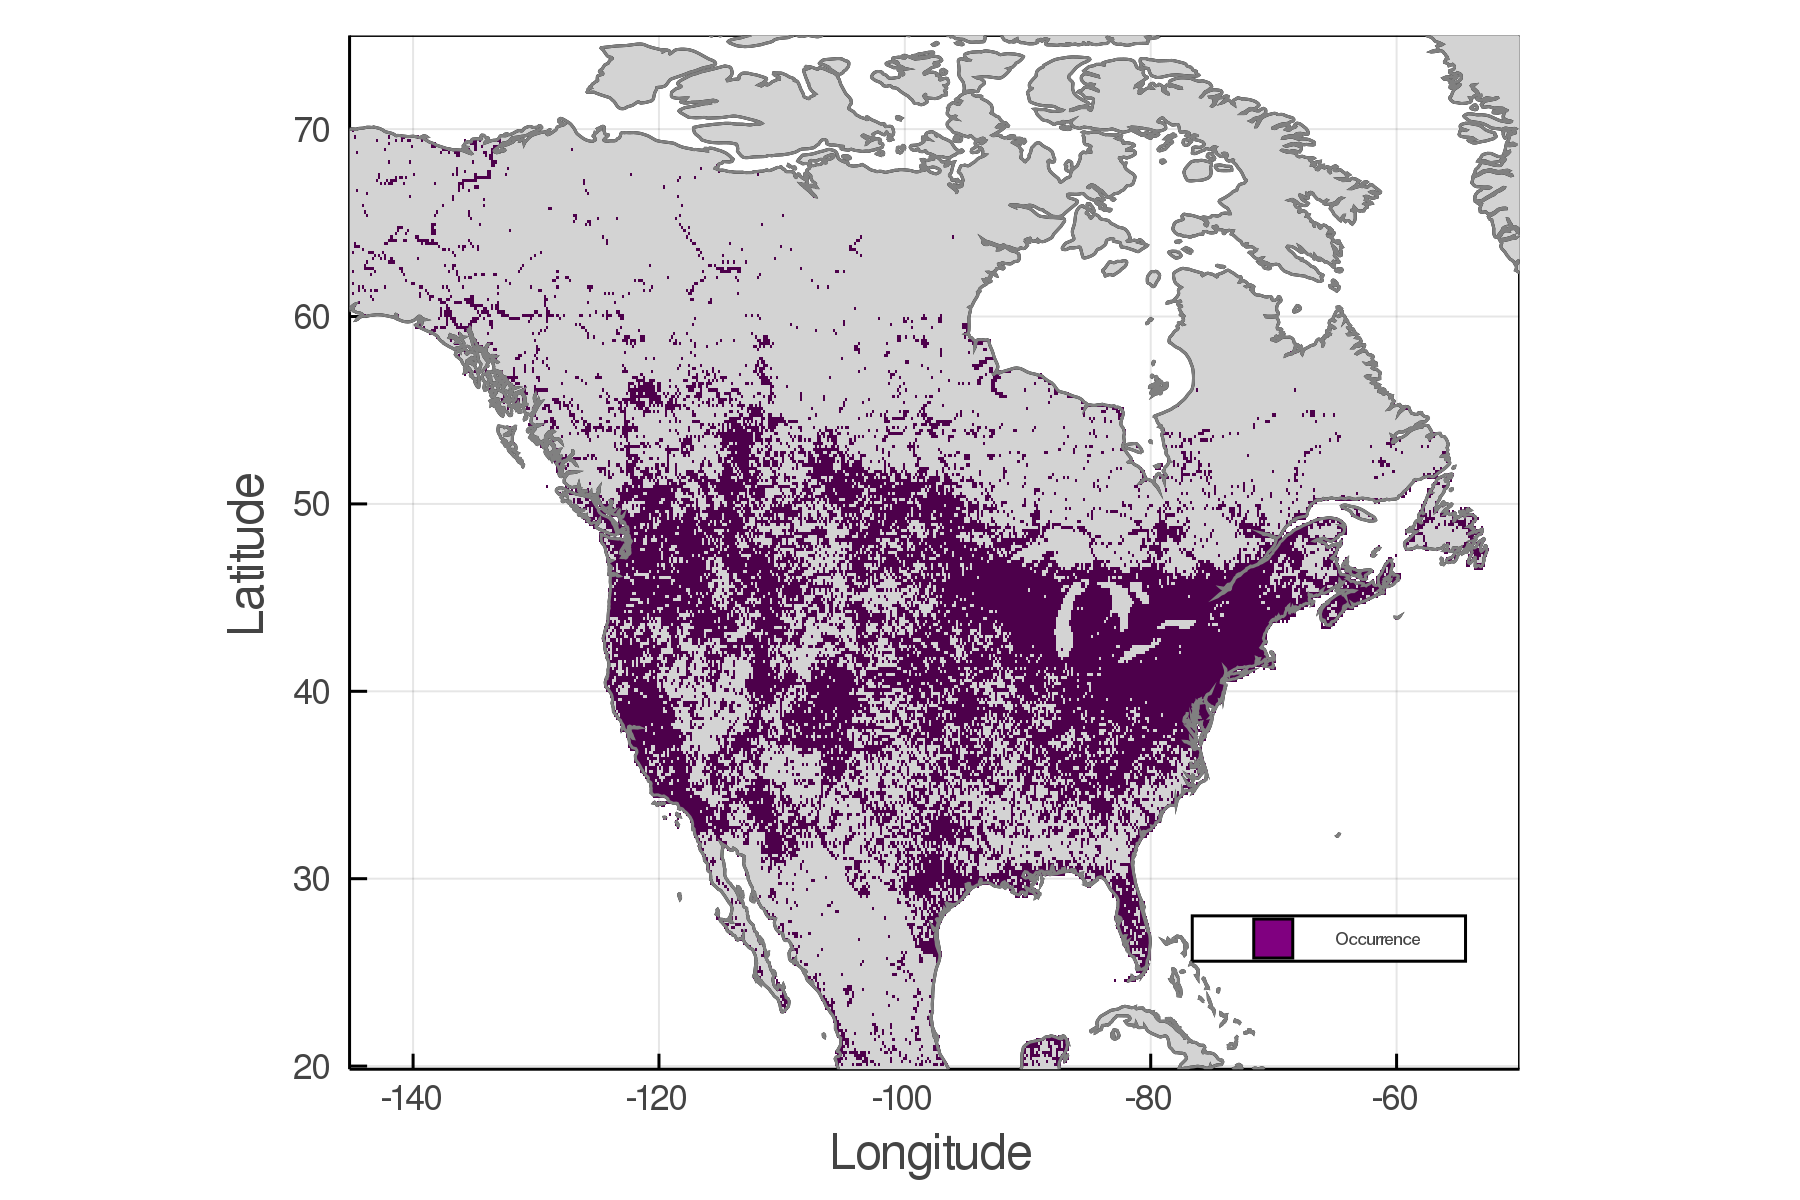
\includegraphics[scale=0.08]{fig/01_raw_singlesp.png}
    \hspace*{0.5cm}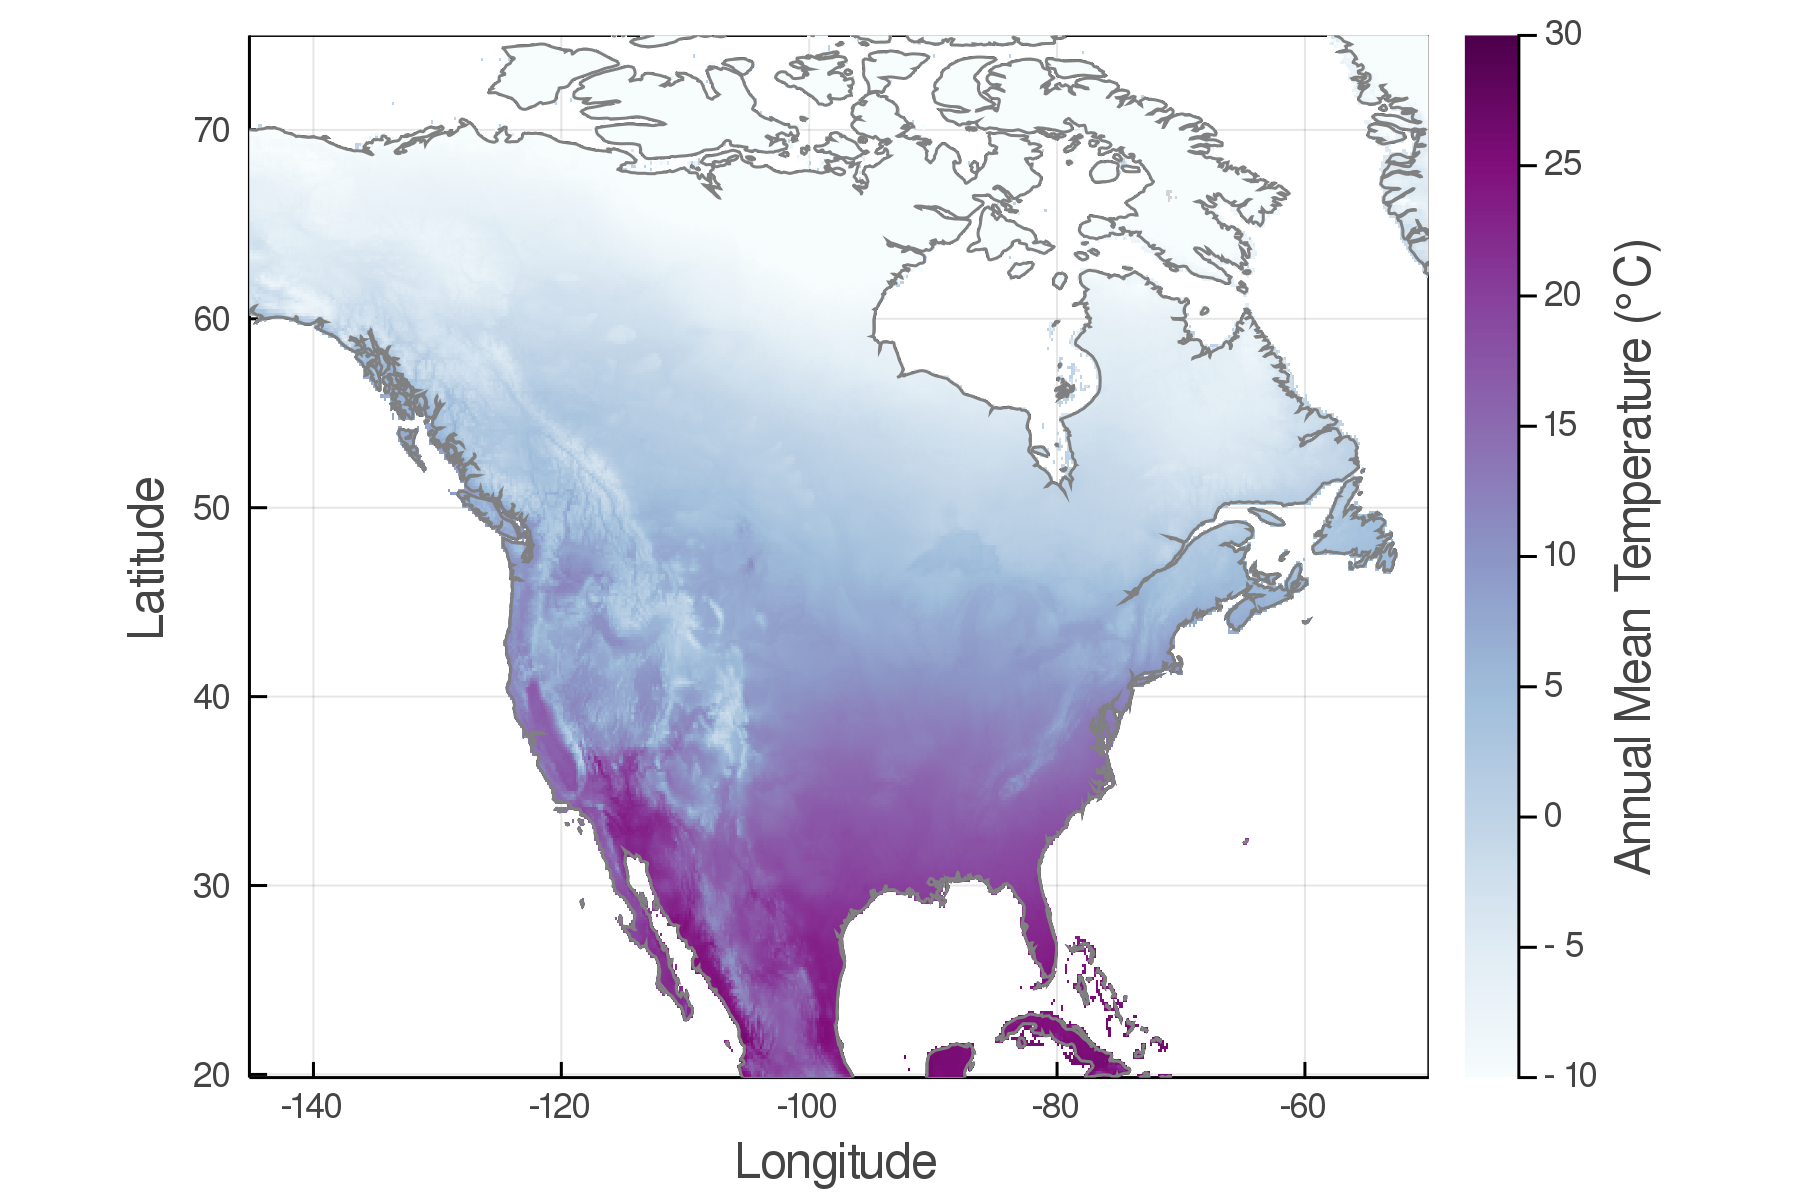
\includegraphics[scale=0.08]{fig/wc_temp.png}
  \end{figure}
\end{frame}

\begin{frame}
  \frametitle{Objective}
  \begin{figure}
    \centering
    \hspace*{-0cm}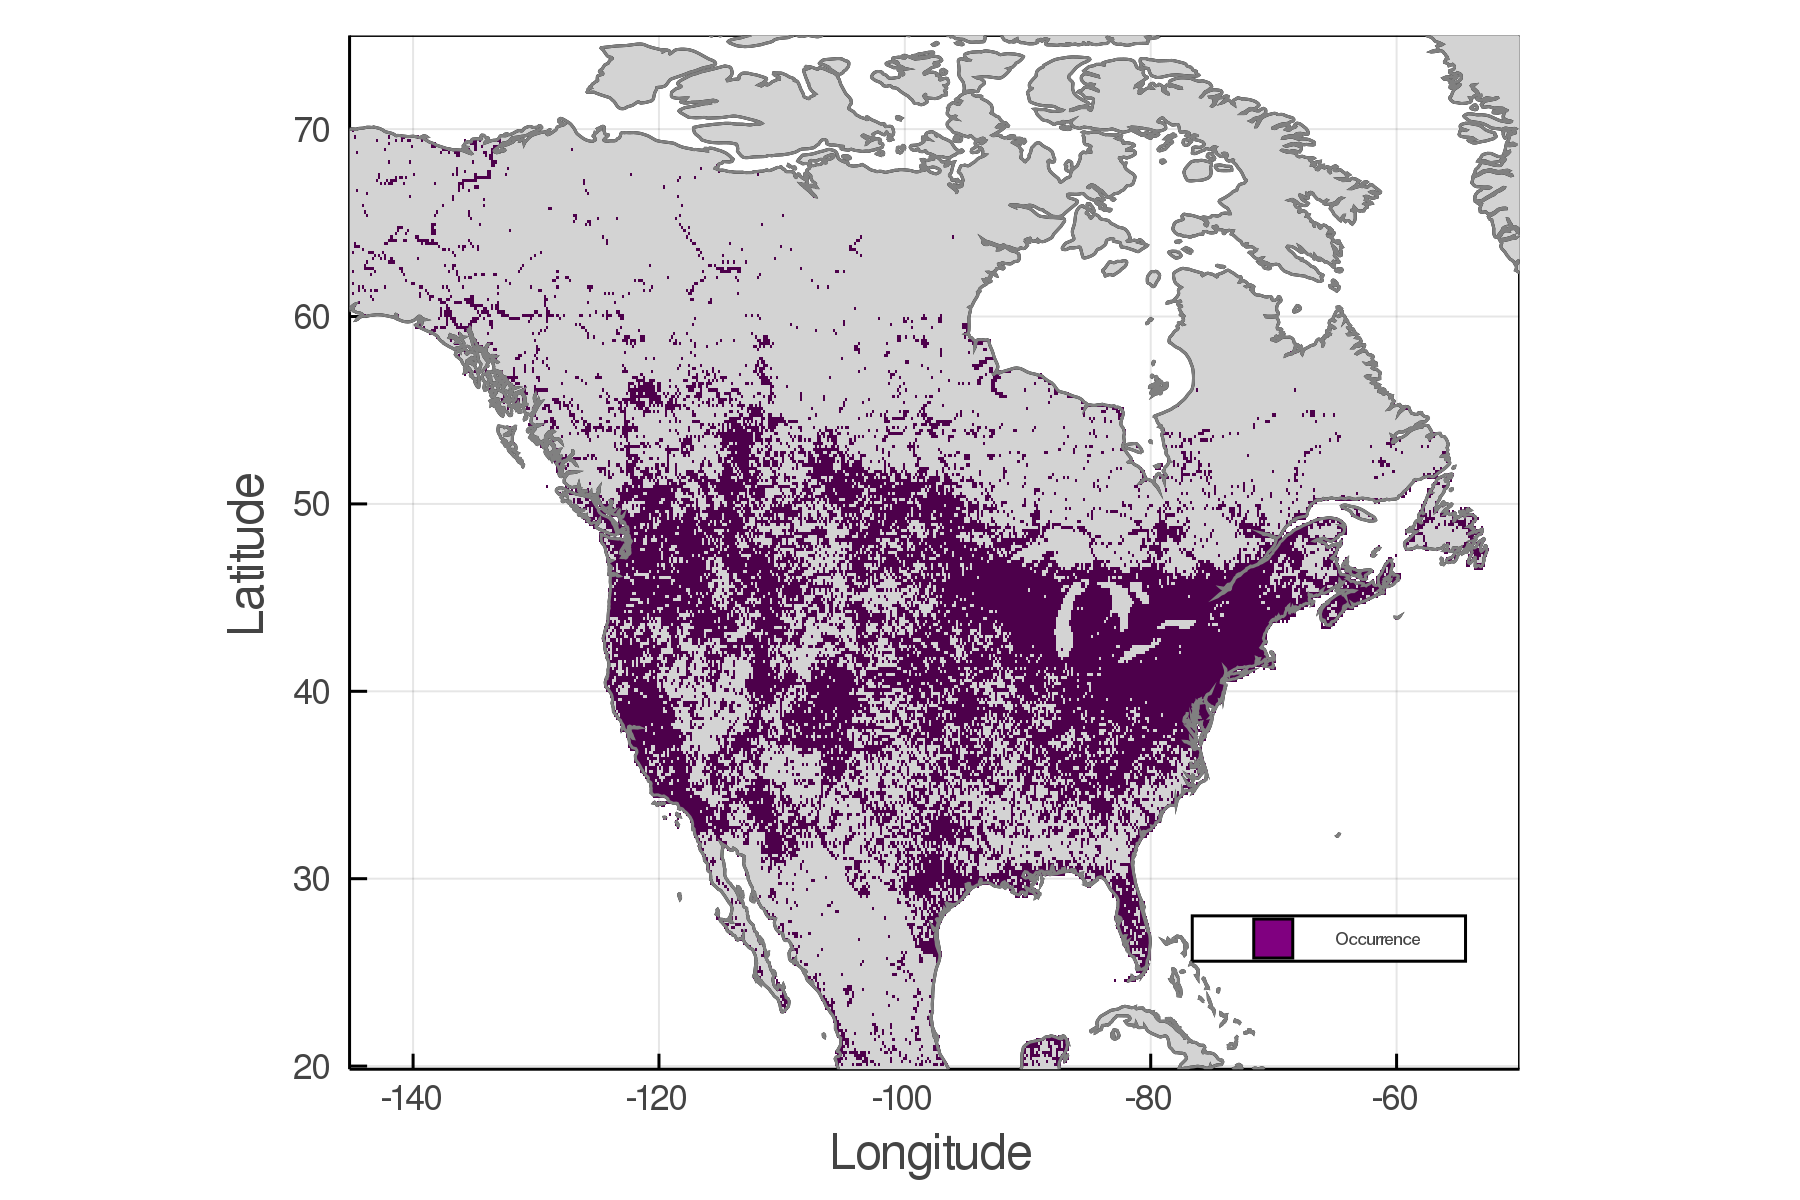
\includegraphics[scale=0.05]{fig/01_raw_singlesp.png}
    \hspace*{0cm}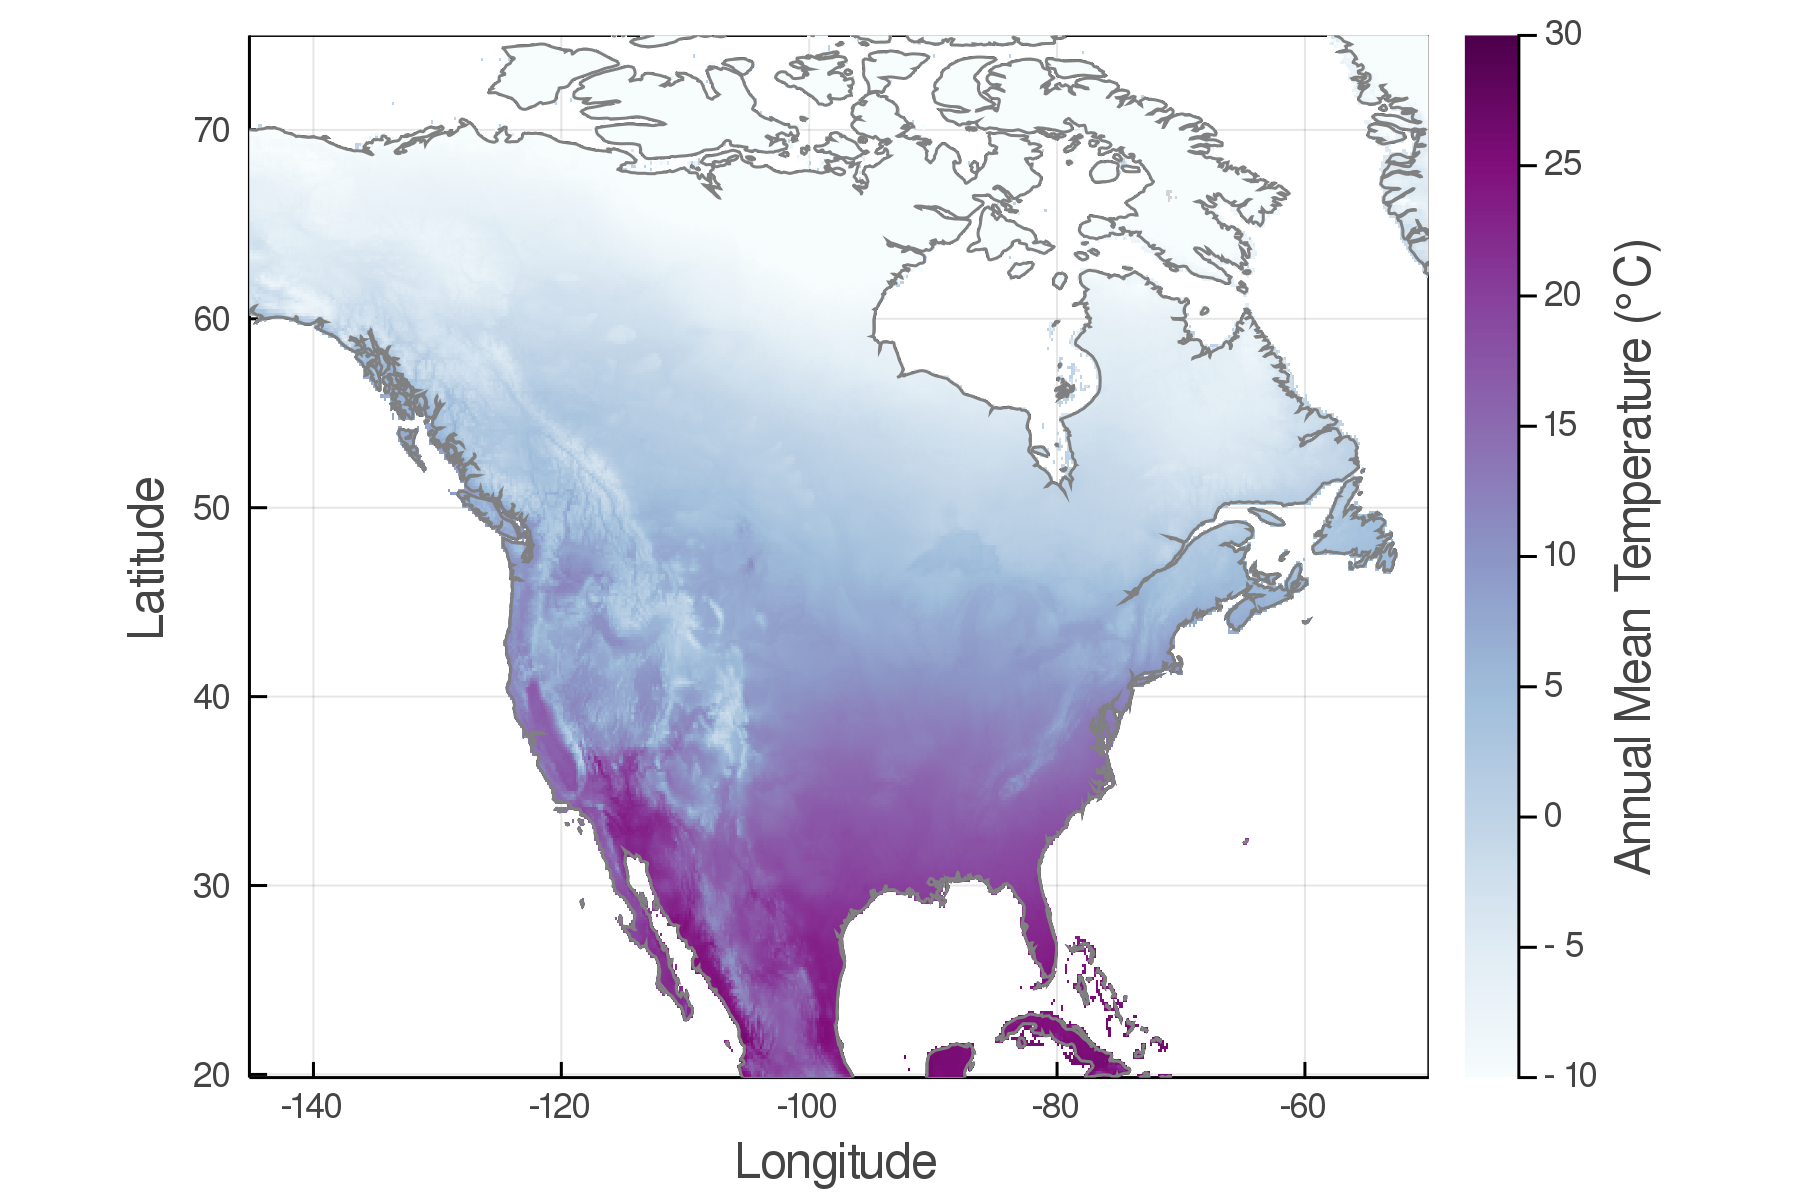
\includegraphics[scale=0.05]{fig/wc_temp.png}
    \vfill
    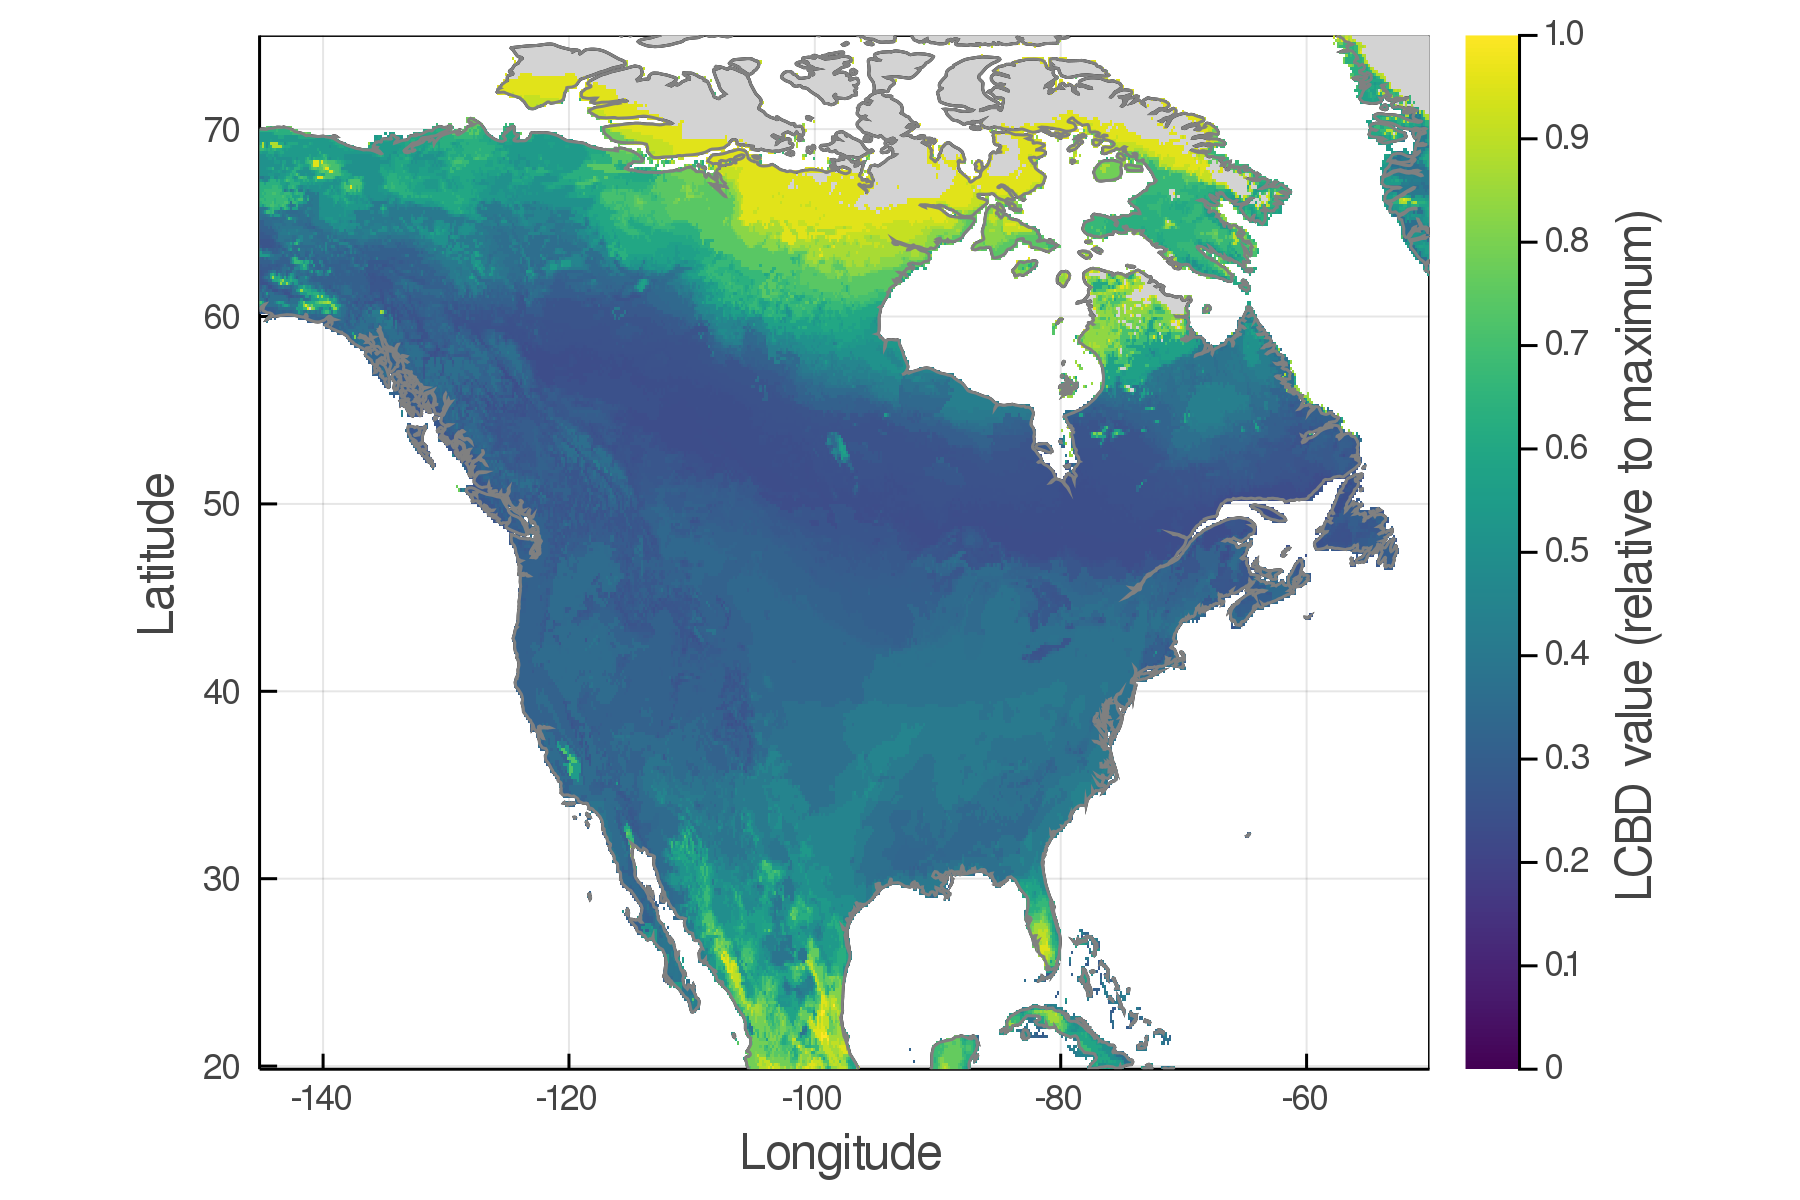
\includegraphics[scale=0.10]{fig/05_sdm_lcbd.png}
  \end{figure}
\end{frame}

\begin{frame}
  \frametitle{Data - Why eBird \& Warblers}
  According to Johnston et al. (2019):
  \begin{enumerate}
    \item Complete checklists to infer absences
    \item Sampling effort metadata to reduce biases
  \end{enumerate}
  \begin{figure}
    \centering
    \caption{Structure of the Warblers (\textit{Parulidae}) occurrence data for North America as checklists in the eBird Dataset}
    \hspace*{-0cm}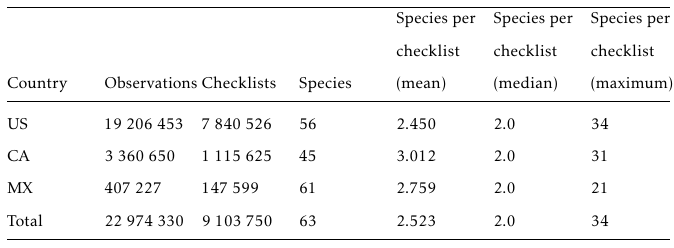
\includegraphics[scale=0.4]{fig/ebird_table.png}
  \end{figure}
\end{frame}

\begin{frame}
  \frametitle{Data - WorldClim 2 (Fik \& Hijmans, 2017)}
  \centering
  \resizebox{0.55\textwidth}{!}{%
    \begin{table}
      \small
      \begin{tabular}{c l}
        \hline
        Variable & Description                            \\
        \hline
        1        & Annual Mean Temperature                \\
        2        & Mean Diurnal Range                     \\
        3        & Isothermality                          \\
        4        & Temperature Seasonality                \\
        5        & Max Temperature of Warmest Month       \\
        6        & Min Temperature of Coldest Month       \\
        7        & Temperature Annual Range               \\
        8        & Mean Temperature of Wettest Quarter    \\
        9        & Mean Temperature of Driest Quarter     \\
        10       & Mean Temperature of Warmest Quarter    \\
        11       & Mean Temperature of Coldest Quarter    \\
        12       & Annual Precipitation                   \\
        13       & Precipitation of Wettest Month         \\
        14       & Precipitation of Driest Month          \\
        15       & Precipitation Seasonality              \\
        16       & Precipitation of Wettest Quarter       \\
        17       & Precipitation of Driest Quarter        \\
        18       & Precipitation of Warmest Quarter       \\
        19       & Precipitation of Coldest Quarter       \\
        \hline
      \end{tabular}
    \end{table}
  }
\end{frame}

\begin{frame}
  \frametitle{BIOCLIM - A Climate Envelope Model}
  \begin{figure}
    \centering
    \hspace*{-0cm}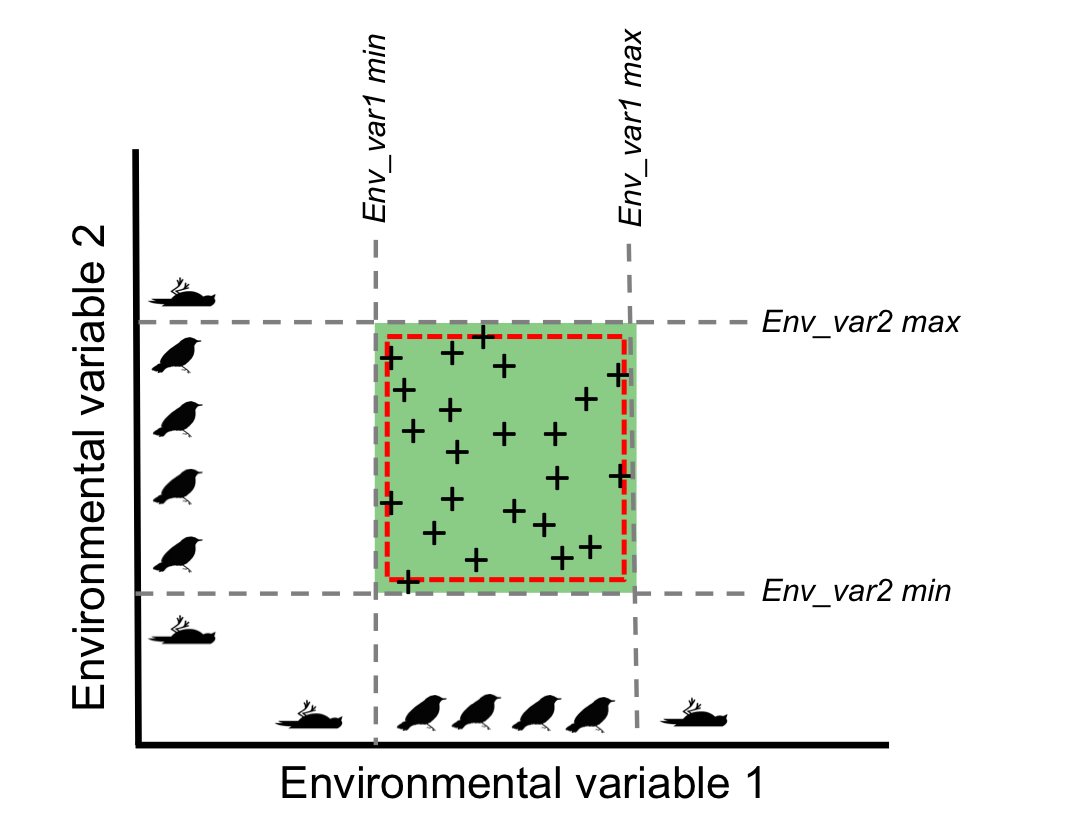
\includegraphics[scale=0.25]{fig/bioclim_bccvl.png}\footnote{\tiny https://support.bccvl.org.au/support/solutions/articles/6000083201-bioclim}
  \end{figure}
\end{frame}

\begin{frame}
  \vfill
  \centering
  \huge Preliminary Results
  \vfill
\end{frame}

\begin{frame}
  \frametitle{Ex. Yellow Warbler - Raw Data}
  \begin{figure}
    \centering
    \hspace*{-0cm}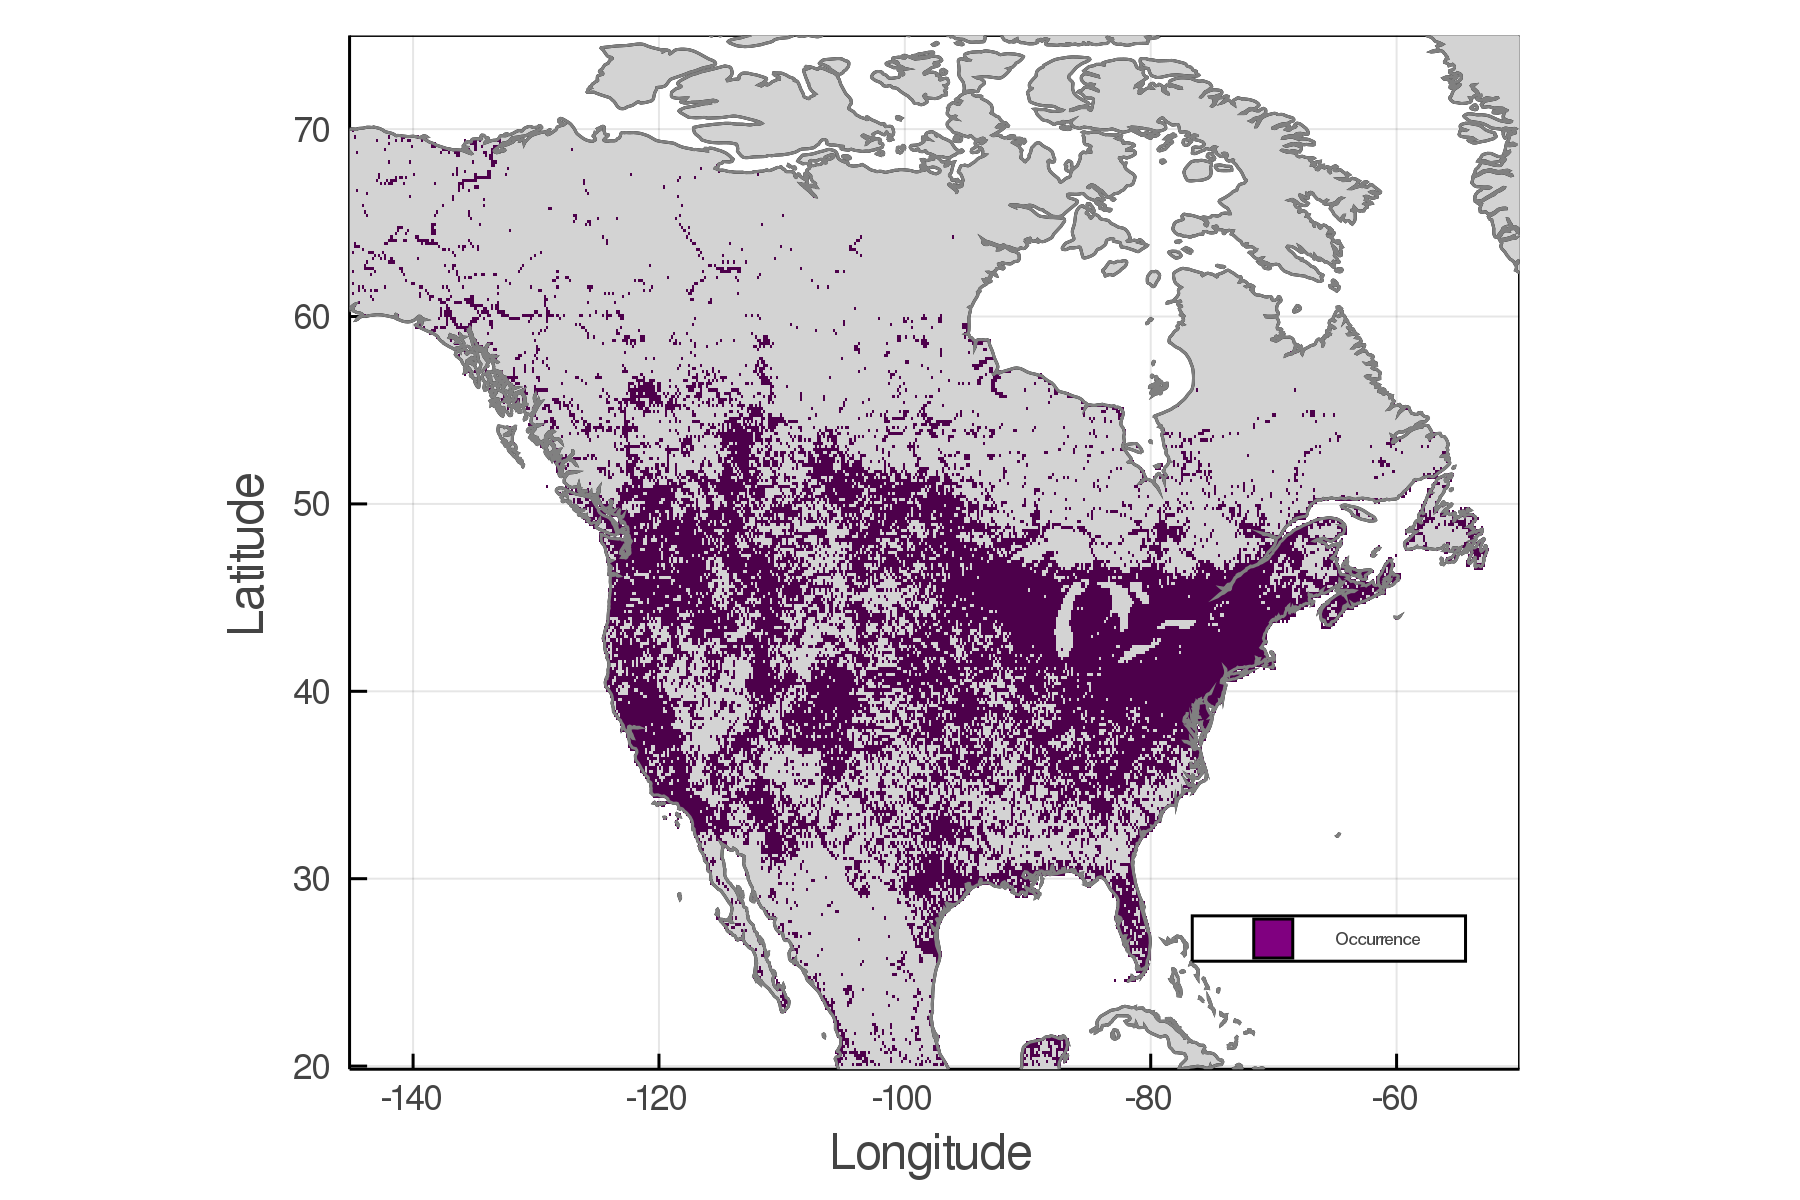
\includegraphics[scale=0.17]{fig/01_raw_singlesp.png}
    \caption{Yellow Warbler Distibution (presence-absence per site)}
  \end{figure}
\end{frame}

\begin{frame}
  \frametitle{Ex: Yellow Warbler - SDM with threshold}
  \begin{figure}
    \centering
    \hspace*{-0cm}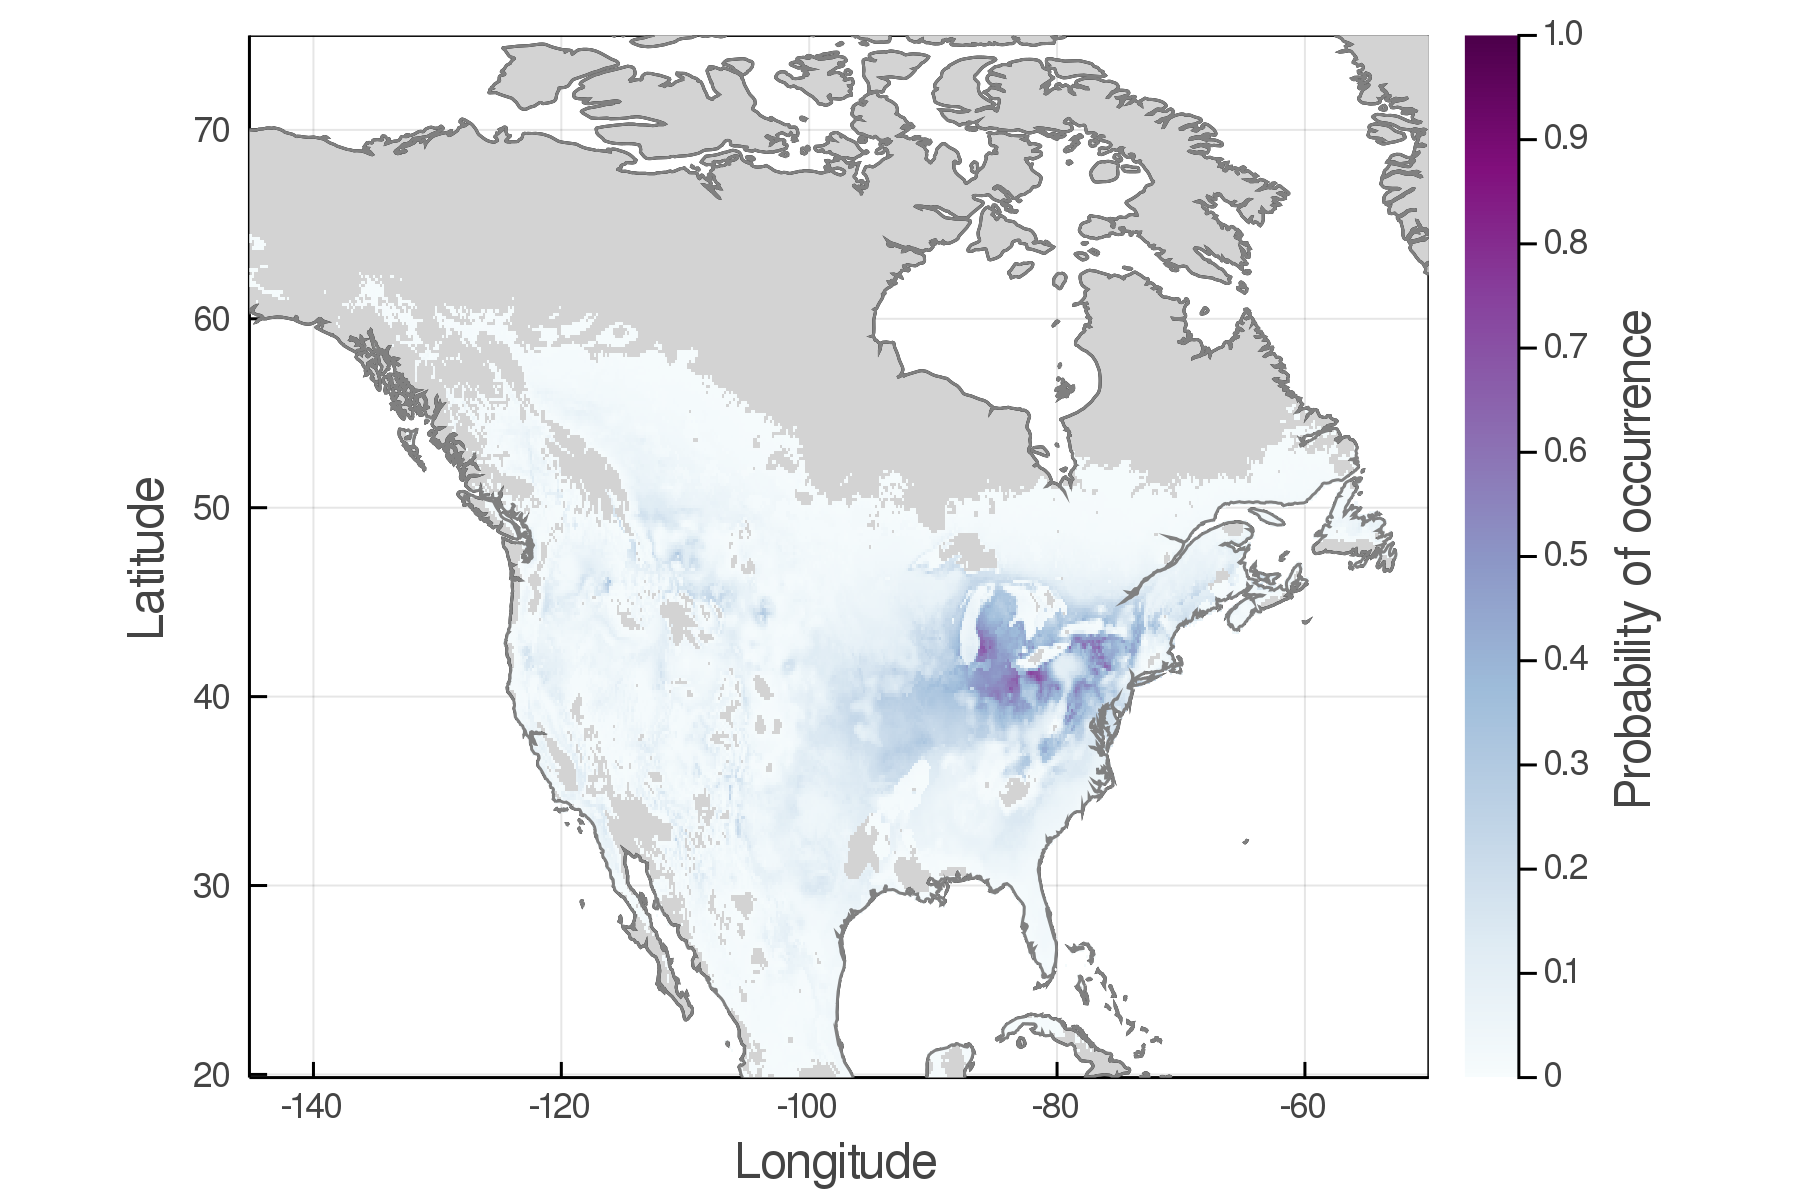
\includegraphics[scale=0.17]{fig/01_sdm_singlesp-threshold.png}
    \caption{SDM predictions with threshold (5\%) for the distribution of Yellow Warblers}
  \end{figure}
\end{frame}

\begin{frame}
  \frametitle{Ex: Yellow Warbler - SDM without threshold}
  \begin{figure}
    \centering
    \hspace*{-0cm}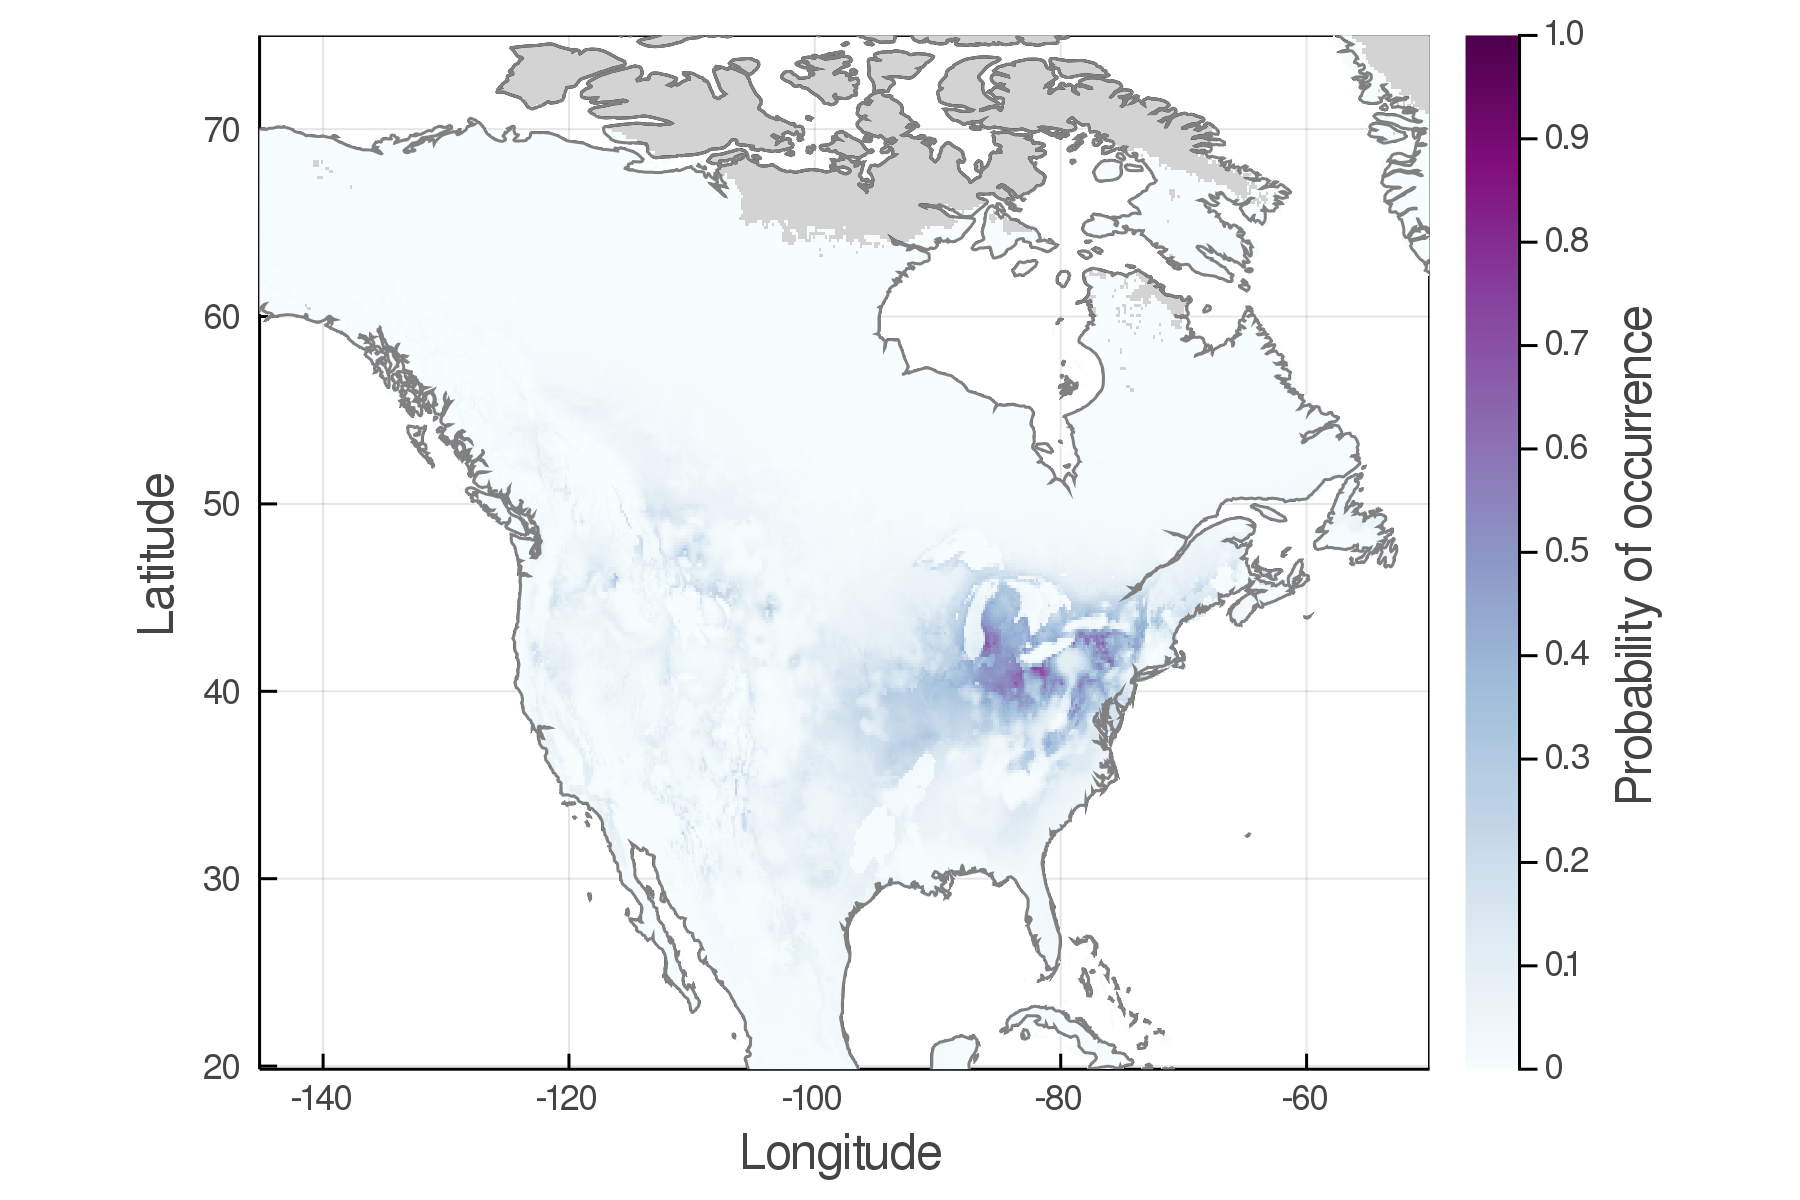
\includegraphics[scale=0.17]{fig/01_sdm_singlesp.png}
    \caption{SDM predictions without threshold for the Yellow Warbler}
  \end{figure}
\end{frame}

\begin{frame}
  \frametitle{Species richness - Raw data}
  \begin{figure}
    \centering
    \hspace*{-0cm}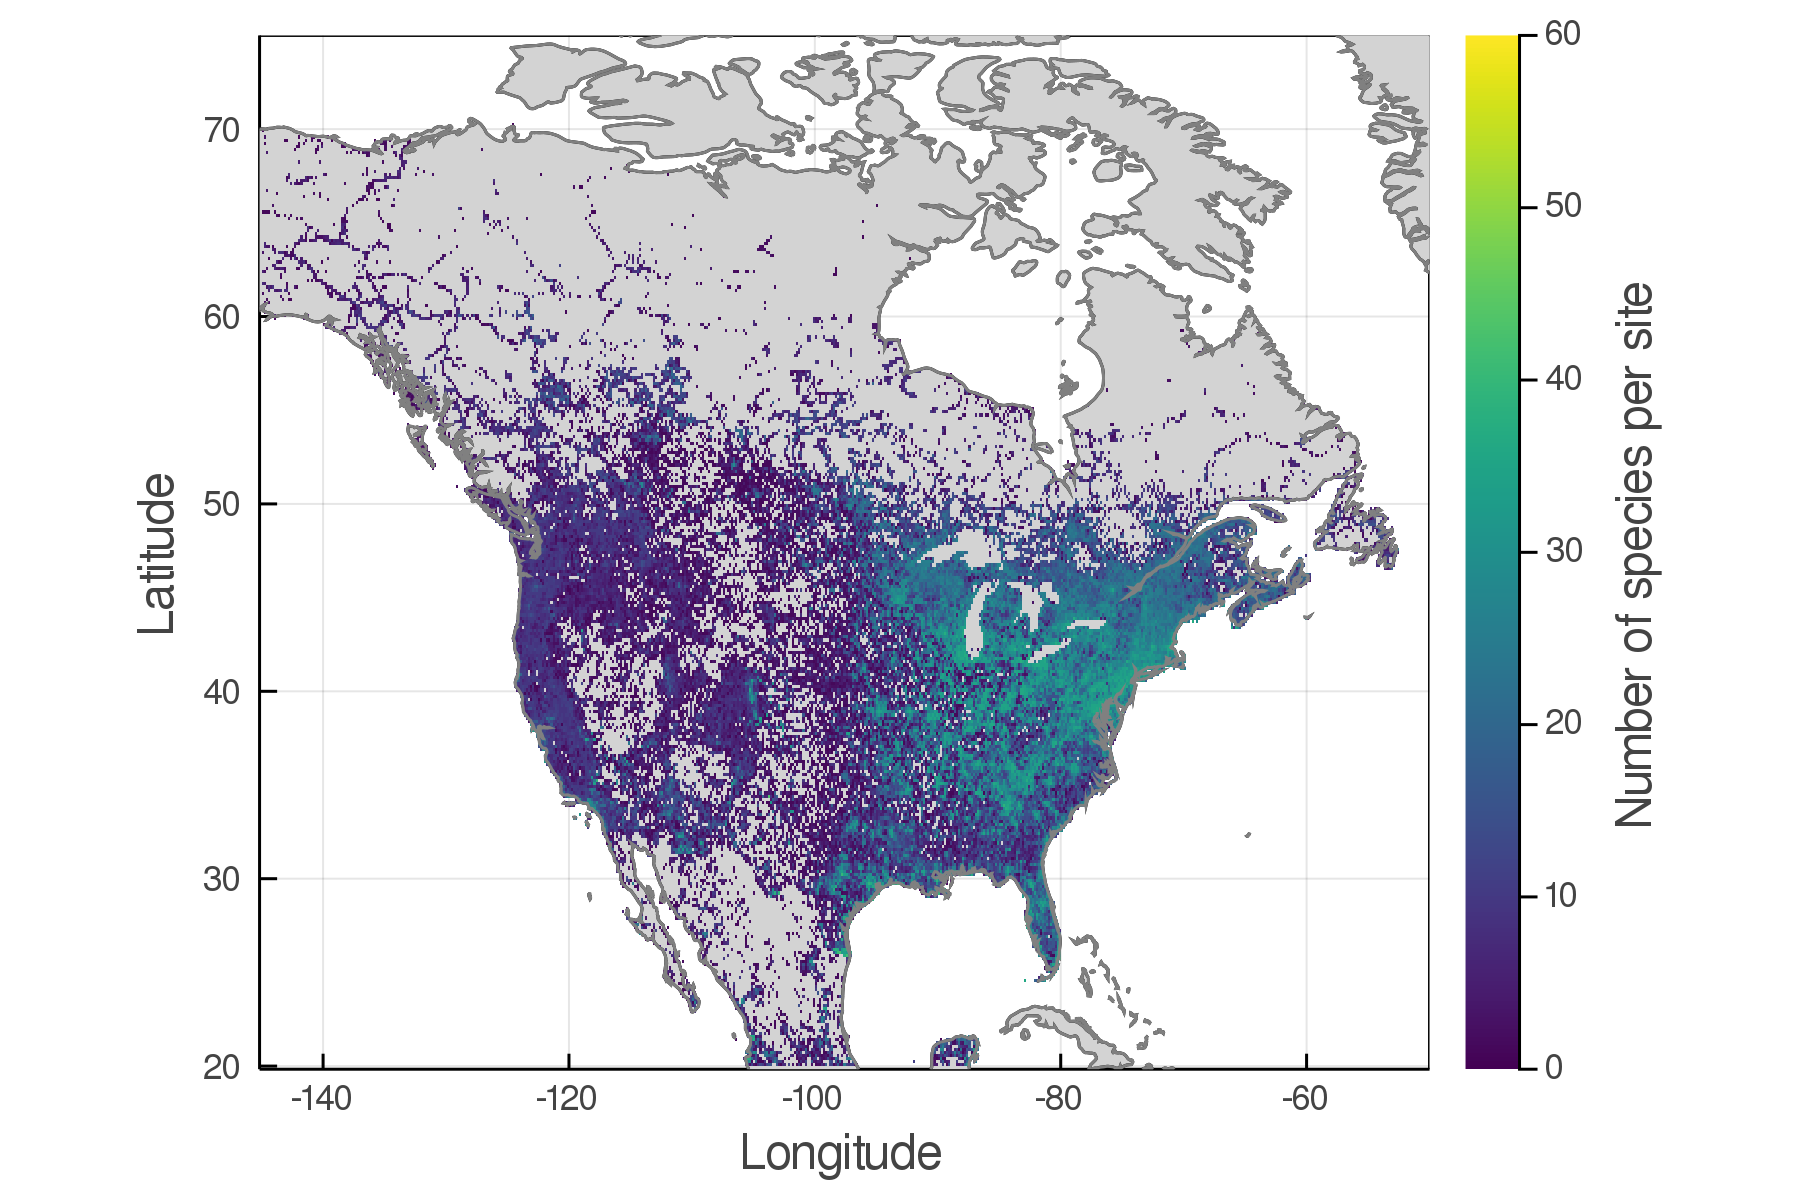
\includegraphics[scale=0.17]{fig/03_raw_richness.png}
  \end{figure}
\end{frame}

\begin{frame}
  \frametitle{Species richness - SDM without threshold}
  \begin{figure}
    \centering
    \hspace*{-0cm}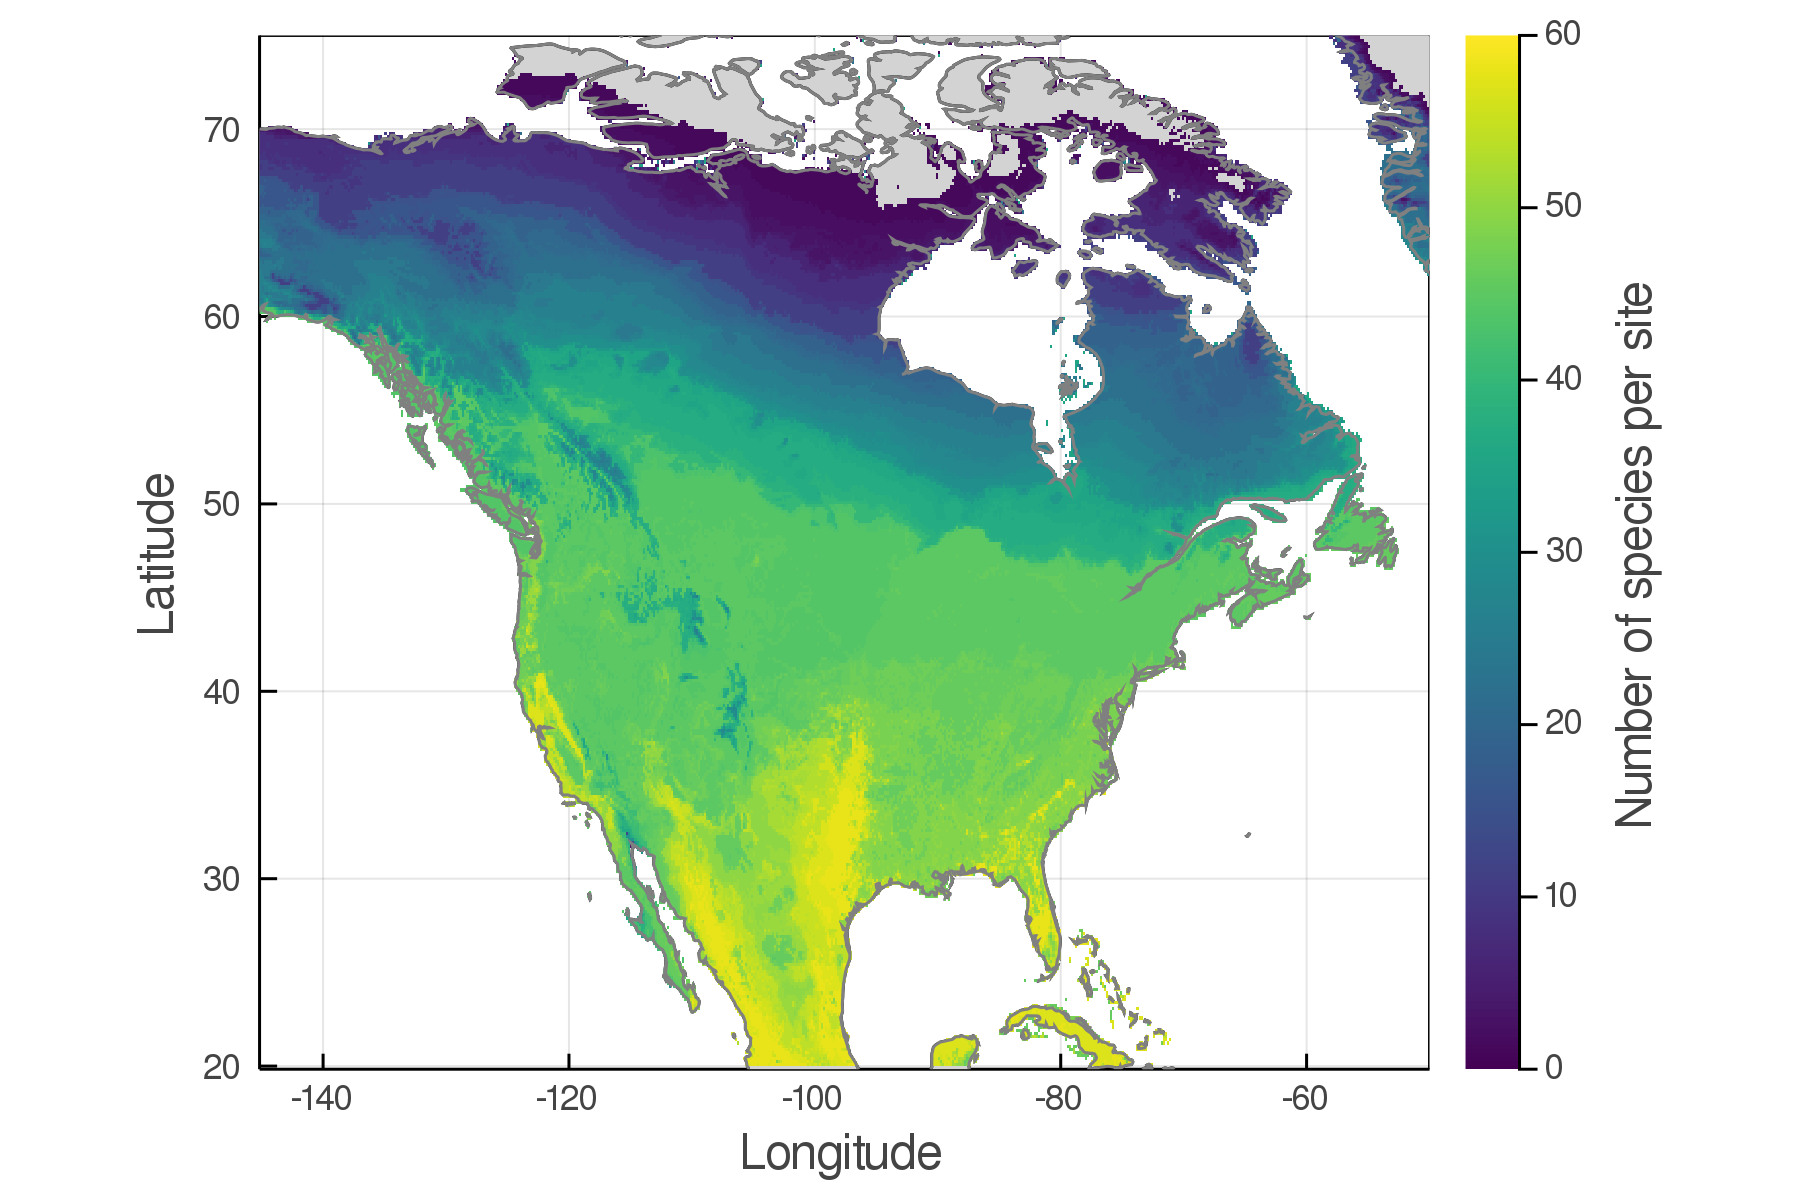
\includegraphics[scale=0.17]{fig/03_sdm_richness.png}
  \end{figure}
\end{frame}

\begin{frame}
  \frametitle{LCBD - Raw data (with Hellinger transformation)}
  \begin{figure}
    \centering
    \hspace*{-0cm}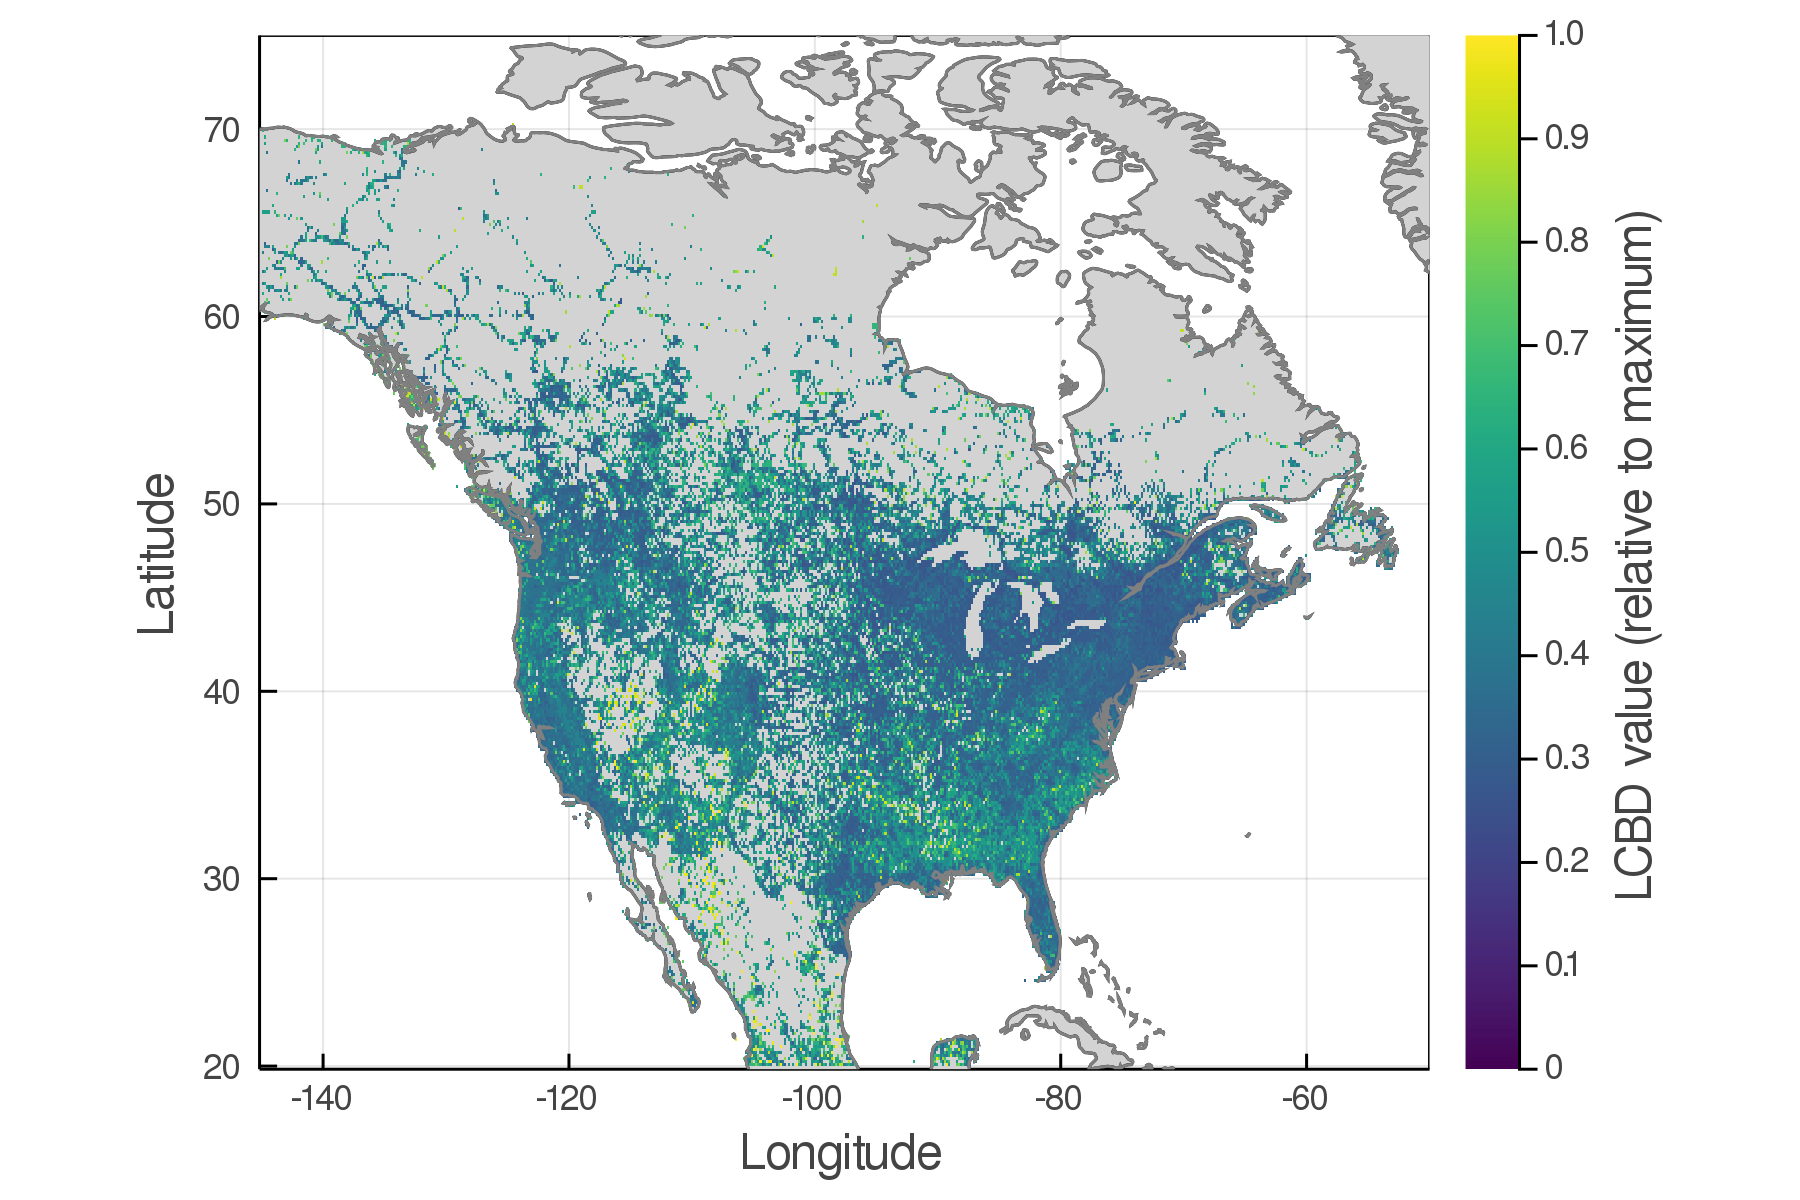
\includegraphics[scale=0.17]{fig/05_raw_lcbd-transf.png}
  \end{figure}
\end{frame}

\begin{frame}
  \frametitle{LCBD - SDM without threshold (no transformation)}
  \begin{figure}
    \centering
    \hspace*{-0cm}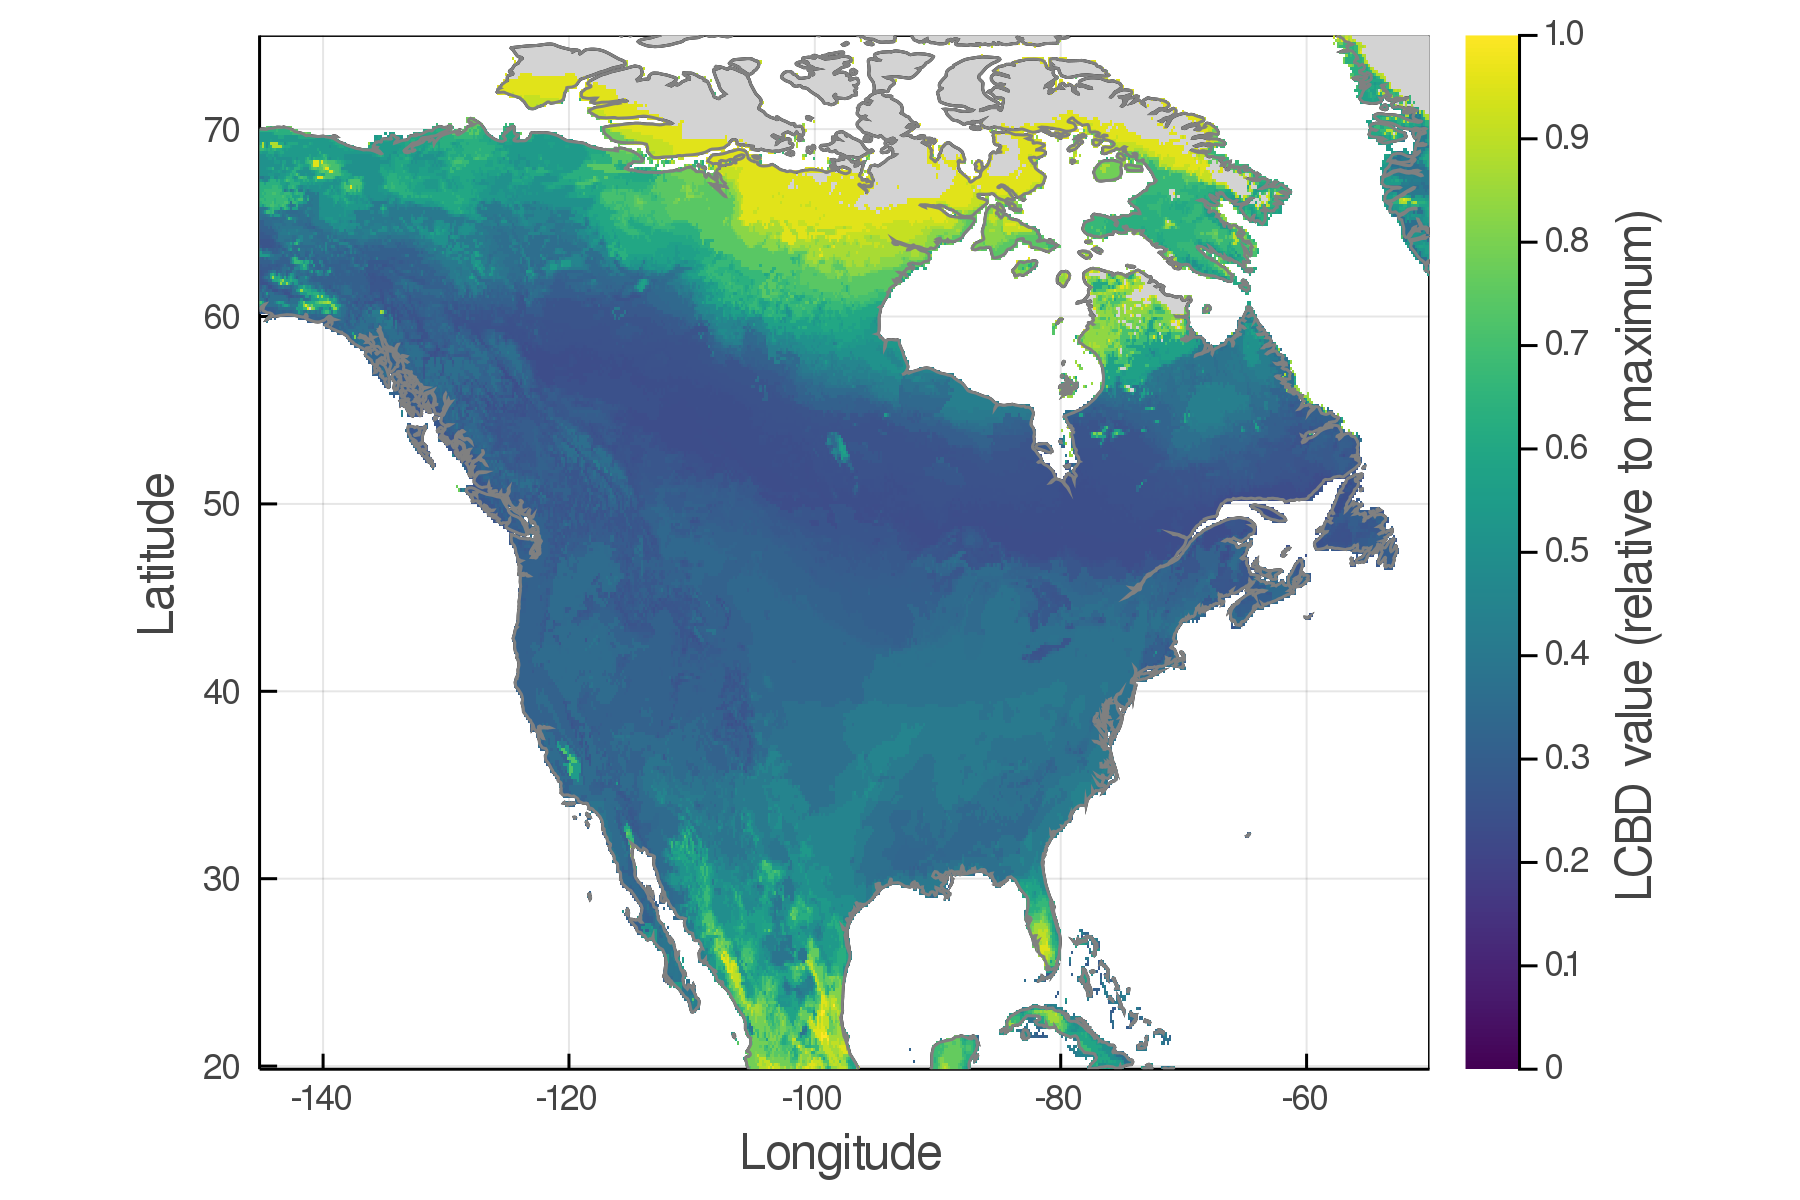
\includegraphics[scale=0.17]{fig/05_sdm_lcbd.png}
  \end{figure}
\end{frame}

\begin{frame}
  \frametitle{LCBD-richness relationship}
  \begin{figure}
    \centering
    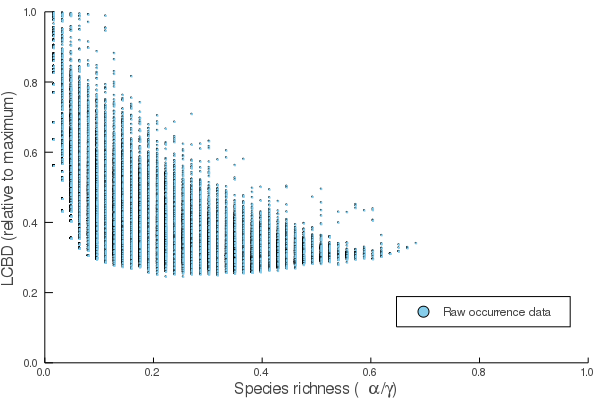
\includegraphics[scale=0.4]{fig/06_raw_relation.png}
  \end{figure}
\end{frame}

\begin{frame}
  \frametitle{LCBD-richness relationship}
  \begin{figure}
    \centering
    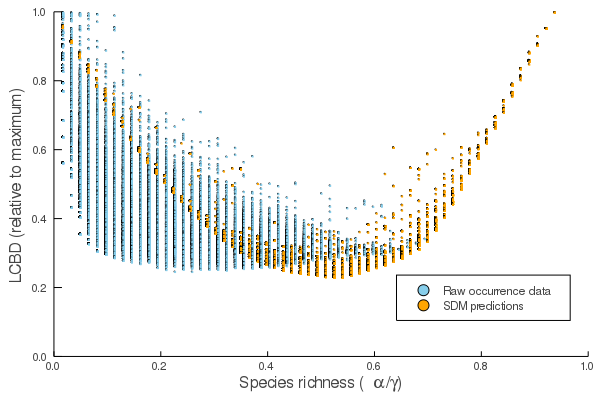
\includegraphics[scale=0.4]{fig/06_cmb_relation-oneplot.png}
  \end{figure}
\end{frame}

\end{document}
